% Syslab Research Journal Template
% By Patrick White
% September 2019

% Do not edit this header
\documentclass[letterpaper,11pt]{article}
\usepackage{fullpage}
\usepackage{palatino}
\usepackage{graphicx}
\def\hrulefill{\leavevmode\leaders\hrule height 20pt\hfill\kern\z@}

% ------------- Edit these definitions ---------------------
\def\name{Bryan Lu}
\def\journalnum{4}
\def\daterange{9/23/19-9/30/19} % starts on Monday
\def\period{2}
% ------------------ END ---------------------------------
% Do not edit this
\begin{document}
	\thispagestyle{empty}
	\begin{flushright}
		{\Large Journal Report \journalnum} \\
		\daterange\\
		\name \\
		Computer Systems Research Lab \\
		Period \period, White
		\end{flushright}
	\hrule height 1pt

% ------ SECTION DAILY LOG -------------------------------------
\section*{Daily Log}
%Detail for each day about what you research, coded, debug, designed, created, etc. Informal style is OK.
\vspace{-0.7em}

\subsection*{Monday, September 23}
\vspace{-0.5em}
I looked through my data set and started to remove the problems that were not actually geometry problems or that were too vague and didn't contain references to specific points/objects. 
\vspace{-1.0em}
\subsection*{Tuesday, September 24}
\vspace{-0.5em}
I finished removing unusable problems from my data set by explicitly searching for capital strings in the line, and started to format the problems I had into a usable form by removing random blank spaces, expanding problems with two parts into two problems, etc. 
\vspace{-1.0em}
\subsection*{Thursday, September 26}
\vspace{-0.5em}
I finished formatting problems by inserting spaces between mathematical operators and symbols and wrote a quick code snippet to find the most common words present in the problems. 

% ------ SECTION TIMELINE -------------------------------------
%\newpage
\vspace{-1.7em}
\section*{Timeline}
\begin{tabular}{|p{1in}|p{2.5in}|p{2.5in}|}
	\hline 
\textbf{Date} & \textbf{Goal} & \textbf{Met}\\ \hline \hline
9/9 & Scrape at least 1000 problems from the AoPS website -- in particular, the High School Olympiads (HSO) forum. & No, but the scraper that I have is nearly functional. Up to scaling, my script can scrape an arbitrary amount of the problems on the page. I did not get many new problems this week.  \\
	\hline
9/16 & Finish writing the webscraper to scrape arbitrarily many problems off of the forums, properly formatted. Begin the process of filtering posts from the dataset. & I was not able to get my webscraper to work, but I've successfully started to format the approximately 300 problems I actually have. \\
	\hline
9/23 & Filter posts that are not standard olympiad geometry problems, and construct a standard lexicon of keywords to look for in a problem both as objects and as relations. & Yes, I created two separate files for various geometrical objects and relations that I found that appeared in my data set. \\
	\hline
9/30 & Write code that creates a graph structure corresponding to the problem statement, with objects as nodes and relations as edges. & N/A  \\
	\hline
10/7 & Research how to write code to create a log-linear classifier and figure out what features of the problem statement should be passed to it. & N/A \\
	\hline 

\end{tabular}


% ------ SECTION REFLECTION  ---------------------------------
\section*{Reflection}
%In narrative style, talk about your work this week. Successes, failures, changes to timeline, goals. This should also include concrete data, e.g. snippets of code, screenshots, output, analysis, graphs, etc.

This week I made decent progress by finishing up my lexicon of words that I would be looking for as well as polishing the problems I did have. I'm ready to start executing the method that I will use to parse the problems and figure out what relations are valid in the context of the problem, using a probabilistic learning method. There are possibly a couple of errant parentheses that will likely make interpretation a bit more difficult, but I'll figure out how to handle this next week. I'm also not sure yet how to handle different forms of a word, but this will something I will also handle next week when I refine my lexicon and identify the objects and relations I want to detect explicitly. 

I didn't filter out the most common words in English, but below is the output file of the most common words in these problems. As expected, the vast majority of these problems revolve around a triangle usually called $ABC$, and a lot of them are $A$-centric, i.e. the problem is framed around lines through $A$ and its opposite side, $BC$. 

\begin{center}
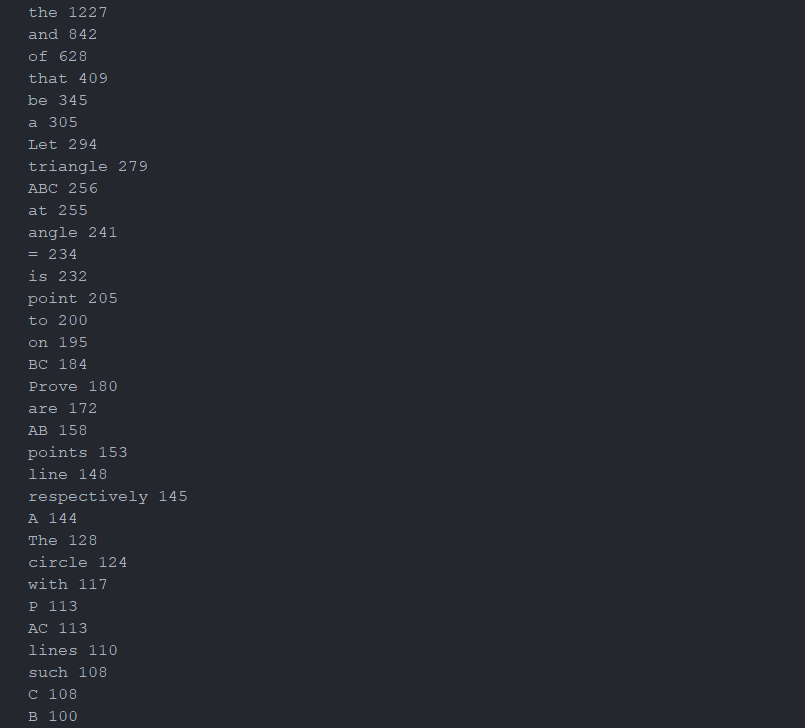
\includegraphics[scale=0.7]{mostcommon.png}
\end{center}



\end{document}

